\title{Bonusaufgabe Bloom-Filter}
\author{
         Severin Peyer, Daniel Obrist\\
}
\date{\today}

\documentclass[12pt]{article}
\usepackage{graphicx}
\usepackage{hyperref}
\graphicspath{ {./images/} }

\begin{document}
\maketitle

\section{Idee des Bloom-Filters}
Der Bloom-Filter ist eine pobabilistische Datenstruktur um schnell und speichereffizient zu bestimmen, ob ein Element in einem Set vorhanden ist. Er kann uns sagen, ob ein Element entweder definitiv nicht im Set ist oder sich mit einer gewissen Fehlerwahrscheinlichkeit im Set befinden kann.

Ein Bloom-Filter ist ein Array von \textit{m} Bits, die anfangs alle auf 0/false gesetzt sind. Wird ein Element in das Set hinzugefügt, werden durch \textit{k} unterschiedliche Hash-Funktionen Hashcodes berechnet. Diese Hashcodes bestimmmen, welche Stellen des Bloomfilters auf 1/true gesetzt werden. So entsteht eine Art Fingerabdruck aller hinzugefügten Daten. Beim Überprüfen ob ein Element enhalten ist werden ebenfalls die Hashcodes des Elements berechnet und mit dem Bloom-Filter verglichen. Wenn an einer der Positionen 0/false steht, ist das Element definitiv nicht im Set. Es können aber False-Positives entstehen, wenn per Zufall zwei Elemente die gleichen Hashcodes generieren.  Je mehr Elemente zur Menge hinzugefügt wurden, desto grösser wird diese Fehlerwahrscheinlichkeit \textit{p}, dass man aus Versehen eine positive Antwort bekommt, obwohl das Element gar nicht im Set enthalten ist.


\paragraph{Vorteile}
\begin{itemize}
\item Zeit, um  Elemente hinzuzufügen oder zu überprüfen, ob ein Element im Set ist konstant, O(k)
\item Benötigen den eigentlichen Speicher/die Daten gar nicht
\item Fehlerwahrscheinlichkeit kann festgelegt werden und durch mehrere Hash-Funktionen oder die Filtergrösse gesenkt werden
\end{itemize}

\paragraph{Nachteile}
\begin{itemize}
\item Kann False-Positives liefern
\item Eigentliche Daten müssen separat abgespeichert werden
\item Elemente entfernen ist mühsam
\end{itemize}

\section{Praxisbeispiele}
Beispiele sind NoSQL-Datenbanken wie BigTable, Apache HBase und Apache Cassandra. Diese Datenbanken verwenden Bloom-Filter für das Nachschlagen eines Schlüssels in einer grösseren Tabelle. Der Bloom-Filter wird dabei der eigentlichen Suche vorgeschaltet um unnötige Suchvorgänge einzusparen. Nur wenn der Wert gemäss Bloom-Filter in der Tablle enthalten sein könnte, wird die aufwändige Suche in den Datenwerten angestossen.

\section{Testen der Fehlerwahrscheinlichkeit}
Um die Zuverlässigkeit des Bloom-Filters zu testen, verwenden wir nach dem Einlesen eine grosse Anzahl Testwerte.
Dabei überprüfen wir in der Methode \textit{testReliability()} und mit einer einfachen \textit{contians()}-Abfrage,
ob die Testwerte (von welchen der Bloom-Filter behauptet, dass sie in der Liste seien) auch tatsächlich in der Liste sind.
Das Verhältnis von diesen False-Positives zu der Gesamtanzahl getesteten Wörtern gibt uns dabei die Zuverlässigkeit.
Diese weicht dabei nie mehr als die voreingestellte Fehlerwahrscheinichekit \textit{p} von 100 Prozent ab, da wir die Filtergrösse \textit{m} und
die Anzahl Hash-Funktionen \textit{k} in Abhängigkeit der Anzahl zu speichernden Wörtern \textit{n} anpassen. \footnote{Quelle der Formeln: \url{https://en.wikipedia.org/wiki/Bloom_filter}}

\[
m = - \frac{n \ln p}{(\ln 2)^2}
\]

\[
k = \frac{m}{n} \ln 2
\]


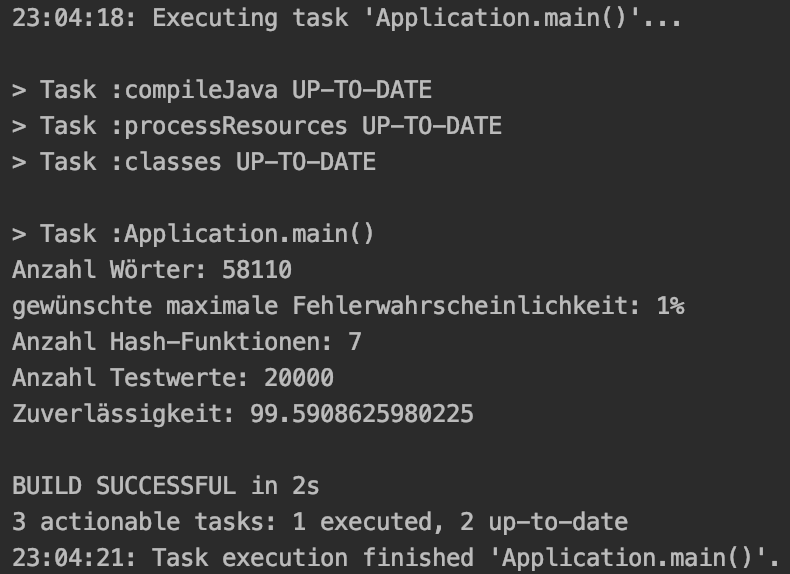
\includegraphics{screenshot}

\end{document}
This is never printed
